\documentclass{beamer}
\usetheme{Madrid}
\usepackage{ragged2e}
\usepackage{listings}


\title{Local Search Strategies for Satisfiability Testing}
\subtitle{GSAT using Random Walk Strategy}
\author{by Oriol Alàs and Joaquim Picó}
\centering
\date{April 2020}
\begin{document}
\maketitle
\begin{frame}
\frametitle{Table of Contents}
\tableofcontents
\end{frame}

\begin{frame}{Introduction}
\framesubtitle{Why have we chosen this paper?}
\section{Introduction}
\textbf{Local Search Strategies for Satisfiability Testing} \\by \textit{Bart Selman}, \textit{Henry Kautz} and \textit{Bram Cohen}.
\linebreak
\begin{itemize}
	\item Our interest raised in:
	\begin{itemize}
		\item  learning some new strategies.
		\item finding out better implementations of GSAT or WalkSAT for our SAT solver.
	\end{itemize}
	\item Wanted to know strategies that mixes the given ones in class.
	\item It talks about simulated annealing and GWSAT strategy.
\end{itemize}
\end{frame}
\begin{frame}{GSAT}
\framesubtitle{Characteristics}
\section{GSAT}
\subsection{Characteristics}
\begin{itemize}
	\item Strategy used for incomplete solvers.
    \item Searches for the "most" satisfiable interpretation. The interpretation that has the maximum number of clauses evaluated to true.
\end{itemize}
\end{frame}
\begin{frame}[fragile]
\subsection{Algorithm}
\begin{verbatim}
for i:=1 to MAX-TRIES
   I := random interpretation for F
   for j:=1 to MAX_FLIPS
      if I satisfies then return I
      Flip any variable in I that
         results in greatest decrease
         in the number o unsatisfied clauses
   end for
end for
return No SAT
\end{verbatim}
\end{frame}
\begin{frame}{GSAT}
\framesubtitle{Advantages and drawbacks}
\subsection{Advantages and drawbacks}
\begin{itemize}
	\item It changes only those literals which have a better number of unsatisfied clause. 
	\item The solver can get stuck in a local optimal in every flip. There are some variations of GSAT to avoid this:
	\begin{itemize}
		\item Using \textbf{restarts}. Creating a new random interpretation every $n$ loop turns.
		\item \textbf{Tabu Search}. Using a data structure that contains all the local optimal already visited. It can be powerful although a high amount of memory is needed in large CNF formulas.
		\item \textbf{Simulated Annealing}.
		\item \textbf{GWSAT}.
		
	\end{itemize}
\end{itemize}
\end{frame}

\begin{frame}{Simulated Annealing}
\section{Simulated Annealing}
\begin{flushleft}

At each step, the \textbf{simulated annealing heuristic }considers some neighbouring interpretation called $i_{new}$ of the current interpretation $i_{current}$.
\\
Probabilistically decides between flip to the neighbour or stay. The function that calculate the probability is determined by:
\end{flushleft}
\begin{itemize}
	\item The current interpretation
	\item The neighbour interpretation
	\item Number of flips already done in the same restart loop iteration.
\end{itemize}
\end{frame}
\begin{frame}{Simulated Annealing in GSAT}
\begin{flushleft}
In order to integrate the simulate annealing algorithm, we can take a reference of this instructions:
\end{flushleft}
\begin{enumerate}
	\item Choose the random variable and get $\delta$\footnote{Cost of flipping}.
	\item If it is a local optimal, flip the variable with probability $e^{-\frac{\delta}{T}}$ where $T$ is the temperature.
	\item Then, reduce the temperature multiplying it by a constant factor ($\textless 1$).
\end{enumerate}
\begin{flushleft}
The main drawback of using this strategy combination is that is very similar with the basic GSAT.
\end{flushleft}
\end{frame}

\begin{frame}[fragile]{Random Walk GSAT}
\framesubtitle{Algorithm}
\section{Random Walk GSAT}
\subsection{Algorithm}
\begin{verbatim}
for i in max_tries:
   for j in max_flips:
      if (probability p):
         pick a variable in some unsat clause
           and flip it in the interpretation
      else:
         follow the standard GSAT scheme 
           -> Make the best possible move
\end{verbatim}
\end{frame}

\begin{frame}{Random Walk GSAT}
\framesubtitle{Results}
\subsection{Experimental Results}
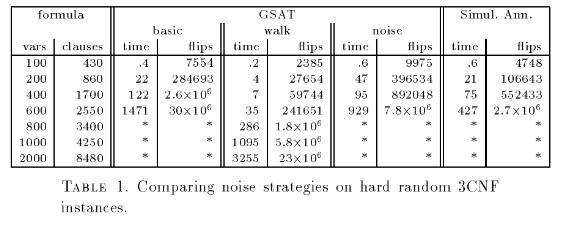
\includegraphics[width=10cm]{imgs/tab1.png}
\begin{itemize}
	\item Little difference in small formulas.
	\item Best performance in largest formulas.
\end{itemize}
\end{frame}
\begin{frame}{Random Walk GSAT}
\framesubtitle{Results}
\subsection{Experimental Results}
Results of max-cut, max-clique, graph coloring, Hanoi or similar problems.
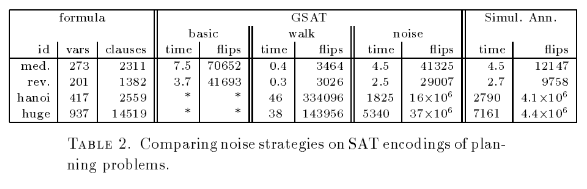
\includegraphics[width=10cm]{imgs/tab2.png}
\end{frame}

\begin{frame}{Random Walk GSAT}
\framesubtitle{Results}
\subsection{Experimental Results}
Resolving problems such as deriving a logical circuit from its input-output behaviour, comparing it with integer-programming method.
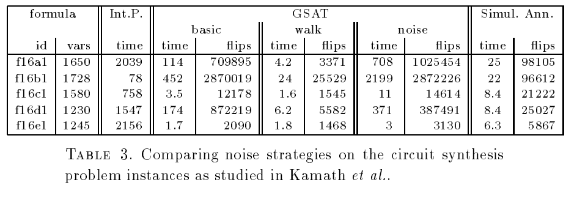
\includegraphics[width=10cm]{imgs/tab3.png}
\begin{itemize}
\item Both GWSAT and SA strategies improve significantly upon GSAT.
\end{itemize}

\end{frame}

\begin{frame}{Random Walk GSAT}
\framesubtitle{Results}
\subsection{Experimental Results}

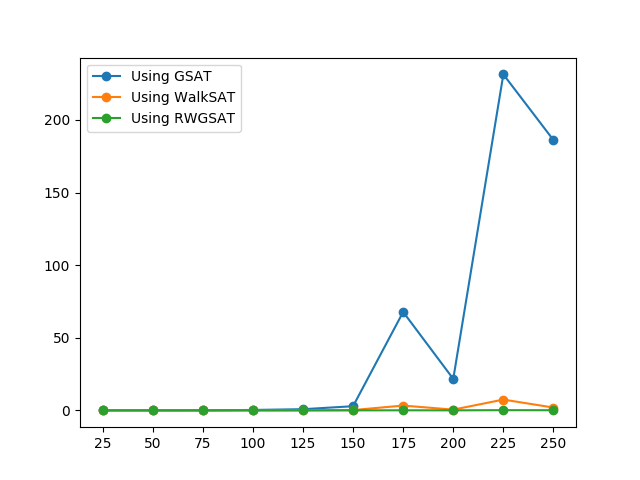
\includegraphics[width=10cm]{imgs/50-graphic-2.png}

\end{frame}
\begin{frame}{Random Walk GSAT}
\framesubtitle{Results}
\subsection{Experimental Results}

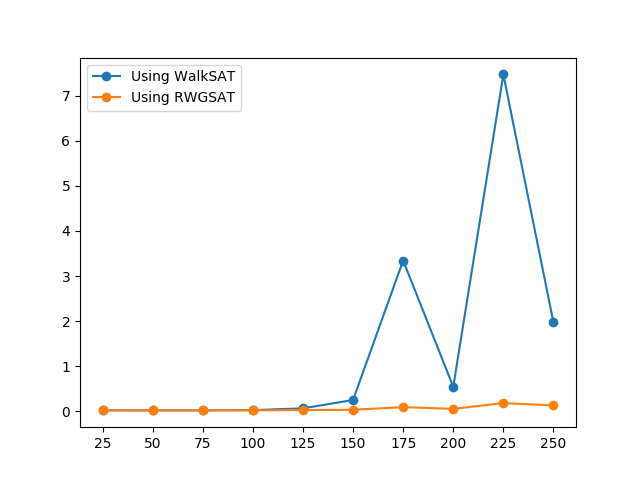
\includegraphics[width=10cm]{imgs/50-graphic-1.png}

\end{frame}
\begin{frame}{Conclusions}
\section{Conclusions}
\begin{itemize}
\item GWSAT is the best option of GSAT variation, including the basic one.
\item We can convert GWSAT into basic GSAT only changing the probability, but not into WalkSAT, because we don't take into account the probability part.
\end{itemize}
\end{frame}
\end{document}
